\documentclass[border=4pt]{standalone}
\usepackage[T1]{fontenc}
\usepackage{lmodern}
\usepackage{amsmath}
\usepackage{pgfplots}
\pgfplotsset{compat=1.18}
\usepgfplotslibrary{groupplots,fillbetween}
\usetikzlibrary{calc,arrows.meta}
% one colour per kind of method, the same in every figure (Okabe-Ito)
\definecolor{neur}{HTML}{D55E00}   % neurons chosen by attribution
\definecolor{dirc}{HTML}{009E73}   % directions from the weird-vs-normal contrast
\definecolor{read}{HTML}{0072B2}   % readout methods and interventions chosen from readouts
\definecolor{pers}{HTML}{CC79A7}   % Assistant Axis / persona
\definecolor{ctrl}{HTML}{8C8C8C}   % random controls
\definecolor{meas}{HTML}{E69F00}   % measured outcome
\definecolor{ink}{HTML}{222222}
\pgfplotsset{
  every axis/.append style={clip=false, font=\small, axis line style={black!55}, tick style={black!55}, tick align=outside,
    label style={font=\small}, tick label style={font=\footnotesize}, title style={font=\small, align=center}},
  grid style={black!9, line width=0.4pt},
  every axis legend/.append style={font=\footnotesize, draw=none, fill=none},
  ci/.style={/pgfplots/error bars/x dir=both, /pgfplots/error bars/x explicit, /pgfplots/error bars/error bar style={line width=0.8pt}, /pgfplots/error bars/error mark=none},
  yci/.style={/pgfplots/error bars/y dir=both, /pgfplots/error bars/y explicit, /pgfplots/error bars/error bar style={line width=0.8pt}, /pgfplots/error bars/error mark=none},
}

\begin{document}
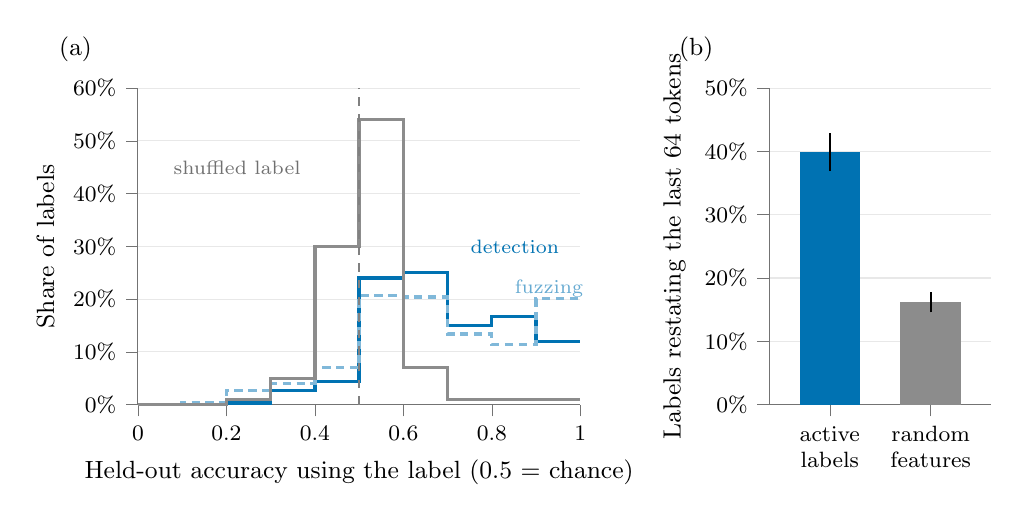
\begin{tikzpicture}
\begin{axis}[name=a, width=7.2cm, height=5.6cm, xmin=0, xmax=1, ymin=0, ymax=60, xtick={0,0.2,0.4,0.6,0.8,1}, xticklabel style={/pgf/number format/.cd, fixed, precision=1}, ytick={0,10,20,30,40,50,60}, yticklabel={$\pgfmathprintnumber{\tick}\%$}, axis x line*=bottom, axis y line*=left, ymajorgrids, xlabel={Held-out accuracy using the label (0.5 = chance)}, ylabel={Share of labels}, title={(a)}, title style={at={(-0.2,1.0)}, anchor=south west}]
\addplot[read, line width=1.2pt] coordinates {(0.00,0.00) (0.10,0.00) (0.10,0.00) (0.20,0.00) (0.20,0.33) (0.30,0.33) (0.30,2.67) (0.40,2.67) (0.40,4.33) (0.50,4.33) (0.50,24.00) (0.60,24.00) (0.60,25.00) (0.70,25.00) (0.70,15.00) (0.80,15.00) (0.80,16.67) (0.90,16.67) (0.90,12.00) (1.00,12.00)};
\addplot[read!50, line width=1.2pt, densely dashed] coordinates {(0.00,0.00) (0.10,0.00) (0.10,0.33) (0.20,0.33) (0.20,2.68) (0.30,2.68) (0.30,4.01) (0.40,4.01) (0.40,7.02) (0.50,7.02) (0.50,20.74) (0.60,20.74) (0.60,20.40) (0.70,20.40) (0.70,13.38) (0.80,13.38) (0.80,11.37) (0.90,11.37) (0.90,20.07) (1.00,20.07)};
\addplot[ctrl, line width=1.2pt] coordinates {(0.00,0.00) (0.10,0.00) (0.10,0.00) (0.20,0.00) (0.20,1.00) (0.30,1.00) (0.30,5.00) (0.40,5.00) (0.40,30.00) (0.50,30.00) (0.50,54.00) (0.60,54.00) (0.60,7.00) (0.70,7.00) (0.70,1.00) (0.80,1.00) (0.80,1.00) (0.90,1.00) (0.90,1.00) (1.00,1.00)};
\draw[black!50, dashed, line width=0.6pt] (axis cs:0.5,0) -- (axis cs:0.5,60);
\node[font=\scriptsize, ctrl!80!black, anchor=east] at (axis cs:0.39,45) {shuffled label};
\node[font=\scriptsize, read, anchor=west, align=left] at (axis cs:0.73,30) {detection};
\node[font=\scriptsize, read!60, anchor=west, align=left] at (axis cs:0.83,22) {fuzzing};
\end{axis}
\begin{axis}[at={($(a.east)+(2.4cm,0)$)}, anchor=west, width=4.4cm, height=5.6cm, ymin=0, ymax=50, xmin=-0.6, xmax=1.6, xtick={0,1}, xticklabels={{active\\labels},{random\\features}}, xticklabel style={align=center, font=\footnotesize}, ytick={0,10,20,30,40,50}, yticklabel={$\pgfmathprintnumber{\tick}\%$}, axis x line*=bottom, axis y line*=left, ymajorgrids, ylabel={Labels restating the last 64 tokens}, title={(b)}, title style={at={(-0.45,1.0)}, anchor=south west}]
\fill[read] (axis cs:-0.3,0) rectangle (axis cs:0.3,39.84);
\fill[ctrl] (axis cs:0.7,0) rectangle (axis cs:1.3,16.15);
\draw[black, line width=0.8pt] (axis cs:0,36.89) -- (axis cs:0,42.97);
\draw[black, line width=0.8pt] (axis cs:1,14.58) -- (axis cs:1,17.87);
\end{axis}
\end{tikzpicture}
\end{document}
